% 经管类标准中文学术论文 LaTeX 模板
% ==========================================

\documentclass[a4paper, 12pt]{article}    % 英文文档类
\usepackage[english]{babel}% 英文断词、标题（Table/Figure）
% ==================== 宏包调用区 ====================
\usepackage[margin=1in]{geometry}    % 页面边距设置为 1 英寸（标准要求）
\usepackage{amsmath, amssymb}        % 数学公式宏包
\usepackage{graphicx}                % 插入图片宏包
\usepackage{booktabs}                % 三线表宏包（配合 Stata 的 esttab）
\usepackage{threeparttable}          % 表格底端加注释宏包（强烈推荐）
\usepackage{multirow}                % 表格合并单元格
\usepackage{makecell}                % 表格内换行
\usepackage{caption}
\usepackage{verbatim}

\renewcommand{\tablename}{Table}
\renewcommand{\figurename}{Figure}
\usepackage{setspace}                % 设置行距
\usepackage[colorlinks=true, linkcolor=blue, citecolor=blue, urlcolor=blue]{hyperref} % 超链接及交叉引用颜色
%\usepackage[numbers, sort&compress]{natbib}
% 改为 APA 风格的 natbib 设置
\usepackage[authoryear, round]{natbib}
\bibliographystyle{apalike}  % 最接近 APA 第 7 版

% 全局行距设置 (1.5倍行距适合盲审和阅读)
\setstretch{1.5}

% 图表标题格式设置
\captionsetup[table]{skip=5pt, font=bf} % 表格标题加粗，与表格距离 5pt
\captionsetup[figure]{skip=5pt, font=bf}
\usepackage{float}

\title{Pricing Volatility Risk in China: A HAR-RV Refined Approach to Term Structure and Asymmetric Predictability }
\begin{comment}
\author{
    Guiyuan Ma$^{1}$ \qquad Zhuangfei Ma$^{1}$ %\qquad Xinfeng Ruan$^{1}$
    \\
    $^{1}$School of Economics and Finance, Xi'an Jiaotong University %\\
    %$^{2}$School of Economics, Another University
}
\end{comment}

\date{}  % 清空日期

\begin{document}

\maketitle

\begin{abstract}
    This paper investigates the pricing of volatility risk in the Chinese market by examining the term structure and asymmetric predictability of the Volatility Risk Premium (VRP). Utilizing 5-minute high-frequency returns and daily option prices of the CSI 300 ETF from 2020 to 2025, we propose a refined approach that integrates the Heterogeneous Autoregressive (HAR-RV) model to optimize VRP construction. Our empirical findings reveal: (1) A distinct intertemporal term structure: the VRP significantly predicts positive ETF returns in the medium term (30–90 days), while this relationship reverses to a significant negative predictor in the long term (120+ days). (2) Asymmetric predictability: positive and negative VRP components exhibit heterogeneous predictive power, with the downside VRP rapidly losing significance over ultra-long horizons (360 days). (3) Methodological superiority: the HAR-RV refined indicator consistently outperforms traditional VRP measures in long-term forecasting. These results highlight the non-linear risk-return dynamics and the unique informational role of option-implied expectations in China's evolving derivatives market.
\end{abstract}
\bigskip

  \par\textbf{Keywords:} Pricing volatility risk; Volatility risk premium (VRP); Return predictability; HAR-RV model; Term structure; Asymmetric effects.
\par\textbf{JEL Classification:} G12; G13; C58
\newpage  % 可选：让目录单独占一页
%\tableofcontents
%\newpage  % 可选：让目录单独占一页

\section{Introduction}

The evolution of China’s capital markets has underscored the critical role of financial derivatives in facilitating price discovery and systematic risk management. A landmark development occurred in December 2019 with the debut of the CSI 300 ETF options, representing the first exchange-traded derivative tied to China’s preeminent broad-based index. Since then, the market has matured amidst a period of profound global instability—characterized by the COVID-19 pandemic, divergent global monetary policies, and escalating geopolitical tensions—all of which have intensified volatility across the A-share landscape. For market participants, these dynamics have effectively transitioned volatility from a latent risk factor into a distinct, tradable asset class \citep{carr2001volatilitytrading}, thereby fueling the demand for sophisticated hedging and pricing mechanisms. Consequently, the CSI 300 ETF options market has emerged as a high-fidelity laboratory for analyzing the pricing of volatility risk. Unpacking the information embedded in this premium is essential not only for refining asset pricing theories in emerging markets but also for understanding the complex, non-linear risk-return trade-offs inherent in China’s financial system.

Volatility stands as a cornerstone of modern financial theory, underpinning the mechanics of asset pricing, portfolio optimization, and risk management \citep{merton1973, engle1982arch}. Beyond the backward-looking nature of historical volatility, the Volatility Risk Premium (VRP)—defined as the wedge between risk-neutral expectations and physical realizations of volatility—captures the premium investors pay to hedge against variance uncertainty. As such, the VRP functions as a potent forward-looking barometer of market risk appetite and latent investor sentiment \citep{bollerslev2009, carr2009variance}. Since the seminal work of \cite{bollerslev2009}, which established the VRP’s robust predictive power for equity returns, this premium has occupied a central position in the discourse on asset pricing. However, while its significance is well-documented in mature markets \citep{bollerslev2014stock}, the unique structural frictions of emerging markets offer a compelling yet under-explored frontier for testing the boundaries of volatility risk pricing.

While the VRP literature in mature markets has established a robust theoretical and empirical consensus—broadly confirming its medium-to-long-term return predictability and its asymmetric pricing of upside versus downside volatility {\citep{bollerslev2014, londono2011variance}}—research within the Chinese context is still evolving {\citep{qiao2024variance}}. To date, domestic studies have predominantly focused on the SSE 50 ETF options or broader spot indices {\citep{chen2009volatility, zheng2013volatility}}. However, comprehensive analyses leveraging long-horizon, high-frequency data since the inception of the CSI 300 ETF options remain notably sparse. Furthermore, existing empirical evidence regarding the direction and persistence of the VRP across different forecasting horizons remains fragmented and occasionally contradictory. Specifically, there is a lack of rigorous exploration into the asymmetric predictive power of partitioned VRP components, and few attempts have been made to refine the VRP’s construction via advanced volatility forecasting models to enhance its predictive efficacy {\citep{timmermann2018forecasting}}. This research gap is further widened by the cessation of China’s official volatility index (iVIX) in 2018, which renders the independent construction of model-free implied volatility {\citep{brittenjones2000, carr2007variance}} not only a theoretical necessity but a practical imperative for capturing the unique risk dynamics of the Chinese market.


To address these issues, this study utilizes a high-frequency dataset comprising 5-minute intraday returns of the CSI 300 ETF and daily option pricing data spanning from January 2020 to October 2025. This comprehensive sample allows for a systematic examination of the VRP’s return predictability, its intricate term structure, and the asymmetric effects embedded in its pricing. A key methodological contribution of this paper is the refinement of VRP construction through the integration of the Heterogeneous Autoregressive (HAR-RV) model {\citep{corsi2012harmodeling}}. By capturing the persistent and multi-component nature of realized volatility {\citep{andersen1998, huang2016modeling}}, this optimized HAR-VRP approach filters out transitory noise and significantly enhances the accuracy of asset return forecasting. Consequently, this research not only broadens the empirical understanding of volatility risk in China’s burgeoning derivatives market but also offers a more robust framework for volatility-based investment strategies.

The contributions of this study are three-fold. First, our analysis offers superior timeliness and institutional relevance by covering the full operational cycle of the CSI 300 ETF options from 2020 to 2025. This period encapsulates diverse market regimes—including the pandemic-induced turbulence and multiple bull-bear transitions—ensuring that our findings are robust to extreme market conditions. Second, we extend the literature on asymmetric volatility pricing {\citep{bollerslev2014}} by decomposing the VRP into its upside and downside components ($VRP^+$ and $VRP^-$). This granular approach unveils the heterogeneous impact of directional volatility risk across various horizons, providing novel empirical evidence of risk-pricing asymmetries in an emerging market. Third, this study achieves a methodological refinement by integrating the HAR-RV model into the VRP framework. By substituting noisy ex-post realizations with more persistent, model-based volatility forecasts {\citep{hansen2010realizedgarch}}, we demonstrate that the optimized HAR-VRP significantly enhances long-term return predictability, offering a more sophisticated toolkit for volatility-based asset allocation.

The remainder of this paper is organized as follows. Section 2 reviews the related literature. Section 3 delineates the construction of the full-sample, positive, and negative VRP indicators and introduces the suite of control variables. Section 4 presents the empirical results from univariate and multivariate regressions, focusing on the term structure and asymmetric influence of VRP components. Section 5 describes the integration of the HAR-RV model and the performance of the optimized HAR-VRP indicator. Section 6 concludes the paper and discusses the implications for asset allocation and risk management.

\section{Literature Review}

The academic discourse on the Volatility Risk Premium (VRP) has evolved from foundational theoretical pricing models to complex empirical investigations in emerging markets. This study situates itself within three interconnected strands of literature: the theoretical mechanism of volatility risk, the informational efficiency of the CSI 300 ETF options, and the methodological refinement of risk premium construction.
\subsection{Theoretical Foundations and International Evidence}
The seminal literature, spearheaded by {\cite{bollerslev2009}} and {\cite{carr2009variance}}, posits that the VRP encapsulates the variance risk appetite of investors and serves as a robust predictor of aggregate equity returns. Theoretically, this predictive power is rooted in the intertemporal capital asset pricing model {\citep{merton1973}} and is closely linked to macroeconomic uncertainty {\citep{drechsler2011, zhou2018variance}}. Empirical evidence from mature markets has broadly confirmed that the VRP carries significant incremental information beyond traditional Fama-French factors {\citep{bollerslev2014stock}}.

Furthermore, recent research emphasizes that volatility risk is not a monolithic construct. {\cite{bollerslev2014}} decomposed realized variation into upside and downside semi-variances, demonstrating that "good" and "bad" volatilities exert asymmetric effects on the risk premium. This line of inquiry has been extended to international contexts, where the VRP is found to resolve global asset pricing puzzles and track the transmission of financial shocks {\citep{londono2017variance, rapach2013}}.

\subsection{The VRP Landscape in China’s Emerging Market}
Research within the Chinese context has gained momentum alongside the launch of various derivatives. Early studies by {\cite{chen2009volatility}} and {\cite{zheng2013volatility}} provided the first systematic evidence that volatility risk is a priced factor in A-shares. The introduction of the CSI 300 ETF options in 2019 represented a regime shift, offering a more liquid and tradable laboratory than previous index-based measures {\citep{huang2016modelfree}}. {\cite{chen2021volatility}} confirmed that the ETF-based VRP is deeply embedded with latent investor sentiment and risk preferences unique to the Chinese institutional environment.

However, emerging markets present unique challenges. {\cite{qiao2024variance}} document that VRP dynamics in emerging economies are often influenced by structural frictions and lower informational efficiency. This is further complicated by the "volatility of volatility" and tail-risk concerns {\citep{chen2018tail, dai2020efficient}}, which necessitate a more granular examination of the VRP across different temporal horizons.

\subsection{Methodological Refinement and Research Gaps}
Despite extensive research, a critical methodological gap persists regarding the construction of the VRP. Most studies rely on ex-post realized volatility as a proxy for physical expectations, ignoring the fact that realized measures are often contaminated by transitory noise {\citep{andersen1998}}. While financial econometrics has long recognized the long-memory properties of volatility {\citep{engle1982arch}}, traditional fractionally integrated models often face identification challenges {\citep{li2022weak}}.

To bridge this gap, \cite{corsi2009} proposed the Heterogeneous Autoregressive (HAR-RV) model... While the HAR-RV framework has been utilized for volatility forecasting \citep{timmermann2018forecasting, huang2016modeling, hansen2010realizedgarch},  its application in refining the VRP to explore the term structure of predictability and asymmetric effects remains sparse, particularly in the CSI 300 ETF market. This study addresses these deficiencies by integrating HAR-RV modeling into the VRP framework, providing a more robust lens through which to view the risk-return dynamics in China.


	% --- 3. 研究设计 ---
\section{Data and Methodology}

\subsection{Sample Selection and Data Sources}
The primary sample for this study comprises 5-minute intraday returns of the Huatai-PineBridge CSI 300 ETF and daily trading records of its corresponding options. The sample period spans from January 2020 to October 2025, a window that captures the full operational cycle of the CSI 300 ETF options market and encompasses diverse market regimes, including the post-pandemic recovery and subsequent structural adjustments in the A-share market.

Intraday high-frequency data were retrieved from the JoinQuant quantitative research platform, while comprehensive option-related metrics—including strike prices, open interest, and mid-quote prices—were sourced from the Wind Financial Terminal. Following the data cleaning protocols established in high-frequency literature {\citep{andersen1998}}, we handled outliers and contract rollover effects to ensure the continuity of the volatility series. All computational tasks and econometric estimations were executed using the Python programming environment.

\subsection{Construction of Volatility Metrics}

\subsubsection{Realized Volatility and Semi-variances}
To capture the persistent dynamics of market fluctuations, we construct the daily realized volatility ($RV_t$) using 5-minute intraday returns. Unlike historical volatility derived from daily closes, $RV_t$ provides a consistent estimator of the quadratic variation of the price process {\citep{andersen1998}}. We define $RV_t$ as follows:
\begin{equation}
RV_t = 100 \times \sqrt{252 \sum_{i=1}^{M} r_{t,i}^2}
\end{equation}
where $r_{t,i}$ is the $i$-th intraday log-return on day $t$, and $M$ is the number of 5-minute intervals. Grounded in the ``good and bad volatility'' framework proposed by {\cite{bollerslev2014}}, we further decompose the total $RV_t$ into upside and downside semi-variances ($RV^+_t$ and $RV^-_t$). This allows us to examine the asymmetric impact of directional price shocks on the risk premium:
\begin{equation}
RV^+_t = 100 \times \sqrt{252 \sum_{i=1}^{M} r_{t,i}^2 \cdot \mathbb{I}_{\{r_{t,i} > 0\}}}, \quad RV^-_t = 100 \times \sqrt{252 \sum_{i=1}^{M} r_{t,i}^2 \cdot \mathbb{I}_{\{r_{t,i} < 0\}}}
\end{equation}
where $\mathbb{I}_{\{\cdot\}}$ denotes the indicator function.

\subsubsection{Model-Free Implied Volatility (MFIV)}
Given the cessation of the official iVIX in 2018, the independent construction of Model-Free Implied Volatility (MFIV) is a practical imperative {\citep{huang2016modelfree}}. Following the methodology of {\cite{brittenjones2000}} and the CBOE VIX white paper, we derive a forward-looking measure of market expectations that does not rely on specific pricing models {\citep{carr2007variance}}:
\begin{equation}
IV^2 = \frac{2}{T} \sum_i \frac{\Delta K_i}{K_i^2} e^{RT} Q(K_i) - \frac{1}{T} \left[ \frac{F}{K_0} - 1 \right]^2
\end{equation}
where $Q(K_i)$ represents the mid-quote price of out-of-the-money (OTM) options at strike $K_i$. To ensure a consistent 30-day horizon, we apply linear interpolation between the two nearest expiration dates. Correspondingly, we construct the directional implied volatilities ($IV^+$ and $IV^-$) to capture asymmetric market anticipations {\citep{bollerslev2009}}.

\subsection{Definition of the Volatility Risk Premium (VRP)}
The central independent variable of this study, the Volatility Risk Premium (VRP), is defined as the wedge between risk-neutral expectations and the physical realization of volatility:
\begin{equation}
VRP_t = IV_t - RV_t
\end{equation}
Following the decomposition logic, we define the positive and negative risk premiums as $VRP^+_t = IV^+_t - RV^+_t$ and $VRP^-_t = IV^-_t - RV^-_t$. While traditional literature often treats the VRP as a monolithic predictor {\citep{bollerslev2009}}, our study explores the heterogeneous predictive power of these partitioned components across various temporal horizons {\citep{bollerslev2014, qiao2024variance}}.

\subsection{Predictive Regression Framework}
To investigate the term structure and asymmetric predictability, we employ the following baseline regression model:
\begin{equation} \label{base}
Ret_{t,t+h} = \alpha_0 + \alpha_1 X_{t} + \boldsymbol{\beta}^\top \mathbf{Control}_{t} + \varepsilon_{t,t+h}
\end{equation}
where $Ret_{t,t+h}$ is the cumulative return over horizon $h \in \{1, \dots, 360\}$. The vector $\mathbf{Control}_{t}$ includes market sentiment and liquidity indicators (e.g., $IV_{MEAN}$, $VOLD$, $IVD$) to ensure the robustness of the VRP signal {\citep{dai2020efficient, zheng2013volatility}}. 
Statistical inference is conducted using Newey-West HAC standard errors \citep{newey1987simple} with lag length set to $h-1$ to correct for heteroskedasticity and overlapping observations-induced moving average serial correlation.

Table \ref{variables} summarizes the control variables utilized to mitigate potential omitted variable bias and enhance the model's explanatory power.

\begin{table}[H]
    \centering
    \caption{Definition of Control Variables}
    \label{variables}
    \renewcommand{\arraystretch}{1.3} 
    \begin{tabular*}{\textwidth}{@{\extracolsep{\fill}}llp{8.5cm}}
        \toprule
        \textbf{Name} & \textbf{Symbol} & \textbf{Operational Definition} \\
        \midrule
        Mean Implied Volatility & $IV_{MEAN}$ & Cross-sectional average of Black-Scholes implied volatilities. \\
        Volume Spread & $VOLD$ & Trading volume difference between call and put options ($VOL_{C}-VOL_{P}$). \\
        IV Spread & $IVD$ & Implied volatility difference ($BSIV_{C}-BSIV_{P}$). \\
        Near-Term IV Spread & $IVDN$ & $IVD$ for near-term option contracts. \\
        Realized Variance Premium & $RIV$ & Difference in squared volatility ($RV^2-IV^2$). \\
        VIX Index & $VIX$ & $\sqrt{\frac{2}{T}\sum_{i}\Delta K_i \cdot \frac{e^{rT}{\color{red}Q}(K_i)}{K_i^2}}$ \\
        Positive VIX & $VIX^+$ & $\sqrt{\frac{2}{T}\sum_{i}\frac{\Delta K_i}{K_i^2}e^{rT}C(K_i)}$ \\
        Negative VIX & $VIX^-$ & $\sqrt{\frac{2}{T}\sum_{i}\frac{\Delta K_i}{K_i^2}e^{rT}P(K_i)}$ \\
        \bottomrule
    \end{tabular*}
\end{table}


\section{Empirical Analysis}

\subsection{Descriptive Statistics and Correlation Analysis}
Table \ref{描述性统计} presents the descriptive statistics for the core variables from January 2020 to October 2025. Several salient features of the Chinese market emerge from the data. 

First, the Volatility Risk Premium ($VRP$) and its directional components ($VRP^+$ and $VRP^-$) exhibit significant negative skewness, with minimum values deviating substantially from their respective means. In contrast, implied volatility metrics such as the $VIX$ remain relatively stable. This discrepancy suggests that extreme fluctuations in the $VRP$ are primarily driven by ``volatility bursts'' in the realized variation ($RV$) of the underlying ETF, rather than radical shifts in risk-neutral expectations. Such dynamics imply that during periods of market distress, realized price fluctuations in the A-share market often far exceed the hedging costs priced into the options market.

Second, the average $VRP$ is positive (5.8368), consistent with the canonical theory that option sellers require a premium for bearing variance risk. However, the presence of excessively low minima indicates that the Chinese market is prone to sudden, realized risk expansions that momentarily overwhelm the pricing capacity of the derivatives market.

\begin{table}[htbp]
\centering
\caption{Descriptive Statistics for Key Variables}
\label{描述性统计}
\footnotesize
\setlength{\tabcolsep}{5pt}
\renewcommand{\arraystretch}{1.2}
\begin{tabular*}{\textwidth}{@{\extracolsep{\fill}}lcccccccc}
\toprule
\textbf{Variable} & \textbf{Count} & \textbf{Mean} & \textbf{Std. Dev.} & \textbf{Min} & \textbf{25\%} & \textbf{50\%} & \textbf{75\%} & \textbf{Max} \\
\midrule
$VRP$      & 1409 & 5.8368  & 5.2577 & -76.1787  & 3.9452  & 6.2886  & 8.3588  & 21.7916 \\
$VRP^+$    & 1409 & 1.4869  & 6.8916 & -157.8062 & -0.1857 & 2.3530  & 4.5907  & 15.4973 \\
$VRP^-$    & 1409 & -2.0137 & 5.8377 & -69.7234  & -5.1510 & -1.0690 & 1.7763  & 10.0709 \\
$VIX$      & 1409 & 19.7528 & 4.4300 & 12.9343   & 16.6058 & 18.8994 & 21.8143 & 44.5193 \\
$VIX^+$    & 1409 & 12.2871 & 3.6245 & 2.4527    & 9.8070  & 11.7086 & 13.8196 & 31.0594 \\
$VIX^-$    & 1409 & 8.3732  & 4.7792 & 0.0001    & 5.6439  & 8.8168  & 11.3495 & 28.4079 \\
$IVD$      & 1409 & 1.7061  & 1.1647 & -0.3091   & 0.8182  & 1.5916  & 2.2285  & 6.1627  \\
$IVDN$     & 1409 & 0.9206  & 0.8415 & -0.0933   & 0.4103  & 0.7399  & 1.0923  & 4.6671  \\
$VOLD$     & 1409 & 1.1346  & 0.6685 & 0.1084    & 0.6969  & 0.9937  & 1.3907  & 5.9516  \\
\bottomrule
\end{tabular*}
\end{table}



\subsection{Univariate Predictive Regressions}
To evaluate the informational content of the VRP for subsequent asset returns, we first estimate a series of univariate baseline regressions across multiple horizons $h$:
\begin{equation} \label{base2}
Ret_{t,t+h} = \alpha_0 + \alpha_i X_{i,t} + \varepsilon_{t,t+h}
\end{equation}
Following the standard literature, we employ Newey-West HAC standard errors \citep{newey1987simple} with lag length set to $h-1$ to account for overlapping observations.

Table \ref{result1} reports the regression results across eight horizons. A striking pattern emerges: the VRP exhibits a distinct ``positive-to-negative'' term structure. In the medium term ($h \in [30, 90]$), the VRP demonstrates significant positive predictability, reflecting a risk-compensation mechanism. Most notably, in the long term ($h \ge 120$), the relationship reverses, with coefficients becoming negative and highly significant ($p < 0.001$). This reversal suggests that while the VRP compensates for variance risk initially, it acts as a signal for mean-reversion or sentiment correction over extended horizons.


    
\begin{table}[htbp]
\centering
\footnotesize % 缩小字号，防止表格过长跑出页面
\caption{Results of the univariate baseline regression model}
\label{result1}
\renewcommand{\arraystretch}{1.3} % 稍微压缩回归表的行距
\begin{tabular}{lcccccccc}
\toprule
&\multicolumn{8}{c}{Number of days of forecast lag: h}\\
\cmidrule(lr){2-9}
& 1    & 7    & 30   &  60  & 90   & 120  & 180  & 360 \\
\midrule
$VRP$ &0.0001 & 0 & 0.0011$^{***}$ & 0.0014$^{***}$ & 0.0014$^{*}$ & -0.0021$^{***}$ & -0.0053$^{***}$ & -0.0061$^{***}$  \\
&(0.197) & (-0.166) & (2.918) & (3.312) & (2.492) & (-4.342) & (-6.891) & (-4.920) \\
$VRP^+$ &-0.0002 & -0.0001 & 0.0003 & 0.0007 & 0.0006 & -0.0014$^{***}$ & -0.0026$^{***}$ & -0.0029$^{*}$  \\
&(-1.231) & (-0.551) & (1.094) & (1.820) & (1.190) & (-4.061) & (-3.949) & (-2.408) \\
$VRP^-$ &0.0001 & -0.0002 & 0.0005 & 0.0004 & 0.0009$^{*}$ & -0.0020$^{***}$ & -0.0027$^{***}$ & -0.0006  \\
&(0.796) & (-1.231) & (1.690) & (0.880) & (2.044) & (-4.346) & (-4.131) & (-0.646) \\
$IV_{MEAN}$ &-0.0012 & 0.0056 & -0.0116 & 0.0202$^{**}$ & -0.0135 & -0.0416$^{***}$ & -0.1238$^{***}$ & -0.1465$^{***}$  \\
&(-1.041) & (1.509) & (-1.950) & (2.612) & (-1.810) & (-4.552) & (-9.235) & (-8.170) \\
$VOLD$ &0.0008 & 0.0005 & -0.0035 & -0.0096$^{**}$ & -0.0103$^{**}$ & -0.0050 & -0.0018 & 0.0025  \\
&(1.645) & (0.453) & (-1.393) & (-2.705) & (-2.852) & (-1.200) & (-0.322) & (0.325) \\
$IVD$ &-0.0005 & -0.0006 & -0.0053$^{**}$ & -0.0051$^{*}$ & -0.0169$^{***}$ & -0.0250$^{***}$ & -0.0398$^{***}$ & -0.0419$^{***}$  \\
&(-1.555) & (-0.729) & (-3.216) & (-2.022) & (-6.323) & (-8.423) & (-11.586) & (-8.524) \\
$IVDN$ & -0.0006& -0.0001 & -0.0044$^{*}$ & -0.0038 & -0.0148$^{***}$ & -0.0222$^{***}$ & -0.0357$^{***}$ & -0.0320$^{***}$ \\
&(-1.417) & (-0.084) & (-2.134) & (-1.183) & (-4.540) & (-6.316) & (-9.136) & (-5.767) \\
$RIV$ &-0.0003 & 0.0003$^{**}$ & -0.0006 & -0.0011 & -0.0007 & 0.0023 & 0.0142$^{***}$ & 0.0149$^{***}$  \\
&(-0.323) & (2.703) & (-0.577) & (-0.800) & (-0.536) & (1.575) & (6.490) & (4.718) \\
$VIX$ &0 & 0.0001 & 0.0013$^{***}$ & 0.0013$^{*}$ & 0.0028$^{***}$ & 0 & -0.0135$^{***}$ & -0.0112$^{***}$  \\
&(0.333) & (0.682) & (3.576) & (2.107) & (6.954) & (-0.060) & (-11.932) & (-12.302) \\
$VIX^+$ &0.0001 & -0.0001 & 0.0013$^{**}$ & 0.0015$^{*}$ & 0.0039$^{***}$ & 0.0001 & -0.0142$^{***}$ & -0.0108$^{***}$  \\
&(0.935) & (-0.390) & (2.920) & (2.133) & (7.346) & (0.130) & (-11.173) & (-9.188) \\
$VIX^-$ &0.0001 & 0 & 0.0010$^{**}$ & 0.0005 & 0.0014$^{**}$ & -0.0009 & -0.0087$^{***}$ & -0.0043$^{***}$  \\
&(0.660) & (-0.004) & (2.775) & (0.963) & (2.900) & (-1.438) & (-11.843) & (-3.472) \\
\bottomrule
\multicolumn{9}{p{16cm}}{\scriptsize \textit{Note:} $t$-statistics are reported in parentheses and are calculated using Newey-West (1987) HAC standard errors with a lag length of $h-1$ to account for serial correlation and heteroskedasticity. The same applies to all subsequent tables .\par \smallskip *, **, and *** denote significance at the 10\%, 5\%, and 1\% levels, respectively. } \\
\end{tabular}
\end{table}
\begin{comment}
\begin{table}[htbp]
\centering
\footnotesize 
\setlength{\tabcolsep}{3pt} 
\caption{Baseline Univariate Regression Results}
\label{result1}
\renewcommand{\arraystretch}{1.2}
\begin{tabular*}{\textwidth}{@{\extracolsep{\fill}}lcccccccc}
\toprule
&\multicolumn{8}{c}{Forecast Horizon ($h$ in days)}\\
\cmidrule(lr){2-9}
Variable & 1 & 7 & 30 & 60 & 90 & 120 & 180 & 360 \\
\midrule
$VRP$ & 0.0001 & 0.0000 & 0.0011$^{**}$ & 0.0014$^{***}$ & 0.0014$^{*}$ & -0.0021$^{***}$ & -0.0053$^{***}$ & -0.0061$^{***}$ \\
 & (0.197) & (-0.166) & (2.918) & (3.312) & (2.492) & (-4.342) & (-6.891) & (-4.920) \\
\addlinespace
$VRP^+$ & -0.0002 & -0.0001 & 0.0003 & 0.0007 & 0.0006 & -0.0014$^{***}$ & -0.0026$^{***}$ & -0.0029$^{*}$ \\
 & (-1.231) & (-0.551) & (1.094) & (1.820) & (1.190) & (-4.061) & (-3.949) & (-2.408) \\
\addlinespace
$VRP^-$ & 0.0001 & -0.0002 & 0.0005 & 0.0004 & 0.0009$^{*}$ & -0.0020$^{***}$ & -0.0027$^{***}$ & -0.0006 \\
 & (0.796) & (-1.231) & (1.690) & (0.880) & (2.044) & (-4.346) & (-4.131) & (-0.646) \\
\bottomrule
\multicolumn{9}{l}{\scriptsize \textit{Note:} $t$-statistics in parentheses. Significance: $^{*}p<0.05, ^{**}p<0.01, ^{***}p<0.001$.}
\end{tabular*}
\end{table}
\end{comment}
\subsection{Multivariate Predictive Regressions}


To account for interactive market effects and isolate the unique information content of the volatility risk premium, we estimate the multivariate baseline model presented in Table \ref{tab:multivariate_baseline}.

The results indicate that the VRP maintains robust incremental predictive power even after controlling for average implied volatility ($IV_{MEAN}$), trading activity ($VOLD$), and option-implied skewness ($IVD$). Notably, the intertemporal sign-reversal remains a dominant feature across the term structure: the VRP coefficient is significantly positive for the 30-day horizon (0.0014, $t=4.351$) but transitions into a significant negative predictor for $h \ge 120$. This evidence reinforces the dual-role hypothesis, wherein the VRP serves as a risk-compensation proxy in the medium term, while functioning as a barometer for sentiment-driven overreaction over longer horizons. 

Furthermore, the model’s explanatory power, evidenced by the Adjusted $R^2$, exhibits a distinct ``hump-shaped'' pattern, peaking at 26.53\% for the 180-day horizon. This suggests that the informational density of the volatility risk premium for forecasting A-share returns is maximized at the semi-annual frequency.


\begin{table}[htbp]
\centering
\footnotesize 
\setlength{\tabcolsep}{3.2pt} 
\caption{Multivariate Predictive Regression: Pricing Volatility Risk}
\label{tab:multivariate_baseline}
\renewcommand{\arraystretch}{1.2}
\begin{tabular*}{\textwidth}{@{\extracolsep{\fill}}lcccccccc}
\toprule
 & \multicolumn{8}{c}{Forecast Horizon ($h$ in days)} \\
\cmidrule(lr){2-9}
Variable & 1 & 7 & 30 & 60 & 90 & 120 & 180 & 360 \\
\midrule
% 核心变量置顶
\textbf{$VRP$} & 0.0001 & -0.0001 & 0.0014$^{***}$ & 0.0011$^{**}$ & 0.0017$^{***}$ & -0.0015$^{**}$ & -0.0030$^{***}$ & -0.0029$^{**}$ \\
 & (0.266) & (-0.523) & (4.351) & (2.806) & (3.782) & (-3.094) & (-3.909) & (-2.613) \\
\midrule
% 控制变量
$IV_{MEAN}$ & 0.0004 & 0.0213$^{***}$ & 0.0055 & 0.0707$^{***}$ & 0.0629$^{***}$ & 0.0756$^{***}$ & 0.0055 & -0.0306 \\
 & (0.238) & (3.912) & (0.614) & (4.680) & (4.173) & (4.678) & (0.276) & (-1.114) \\
\addlinespace
$VOLD$ & 0.0008 & 0.0007 & -0.0027 & -0.0093$^{**}$ & -0.0101$^{**}$ & -0.0051 & -0.0039 & -0.0004 \\
 & (1.695) & (0.552) & (-1.091) & (-2.671) & (-2.881) & (-1.270) & (-0.826) & (-0.061) \\
\addlinespace
$IVD$ & -0.0007 & -0.0049$^{***}$ & -0.0106$^{***}$ & -0.0178$^{***}$ & -0.0310$^{***}$ & -0.0374$^{***}$ & -0.0215$^{***}$ & -0.0314$^{***}$ \\
 & (-1.528) & (-3.736) & (-4.590) & (-4.072) & (-6.255) & (-6.512) & (-3.630) & (-3.517) \\
\addlinespace
$VIX$ & 0.0001 & 0.0000 & 0.0021$^{***}$ & 0.0006 & 0.0029$^{***}$ & 0.0007 & -0.0116$^{***}$ & -0.0079$^{***}$ \\
 & (0.628) & (0.135) & (5.324) & (0.919) & (5.949) & (0.972) & (-10.298) & (-7.453) \\
\midrule
Observations & 1409 & 1409 & 1409 & 1409 & 1409 & 1409 & 1409 & 1409 \\
Adj. $R^2$ & 0.0024 & 0.0094 & 0.0404 & 0.0276 & 0.0679 & 0.0759 & 0.2653 & 0.1404 \\
\bottomrule
\multicolumn{9}{l}{\scriptsize \textit{Note:} See notes to Table \ref{result1}. *, **, and *** denote significance at the 10\%, 5\%, and 1\% levels, respectively.} \\
%\multicolumn{9}{l}{\scriptsize \textit{Note:}$t$-statistics in parentheses are based on Newey-West HAC standard errors (lag = $h-1$).} \\
\end{tabular*}
\end{table}


\section{Empirical Refinement via the HAR-VRP Model}

\subsection{The HAR-RV Specification}
The Heterogeneous Autoregressive model for Realized Volatility (HAR-RV), pioneered by {\citep{corsi2012harmodeling}}, serves as a cornerstone for modeling the long-memory properties of financial volatility. Grounded in the \textit{Heterogeneous Market Hypothesis}, the model posits that market participants possess distinct trading horizons—ranging from intraday speculators to long-term institutional investors—each contributing to unique volatility components. By linearly superimposing realized volatility across daily, weekly, and monthly scales, the HAR-RV model effectively replicates the observed slow decay in volatility autocorrelation {\citep{andersen1998}}. 

In this study, we implement the following general form of the HAR-RV model to extract the persistent component of physical volatility:
\begin{equation}
RV_{t+1} = \beta_0 + \beta_d RV_t + \beta_w RV_{t,w} + \beta_m RV_{t,m} + \varepsilon_{t+1}
\end{equation}
where $RV_{t,w} = \frac{1}{5} \sum_{i=0}^{4} RV_{t-i}$ and $RV_{t,m} = \frac{1}{22} \sum_{i=0}^{21} RV_{t-i}$ denote the weekly and monthly average realized volatilities, respectively. Leveraging the predicted realized volatility ($\widehat{RV}_{HAR}$), we construct the refined HAR-VRP ($HVRP$) indicators, which filter out transitory high-frequency noise and better isolate the structural risk premium.

\subsection{Predictive Performance of the Univariate HAR-VRP Model}
To evaluate the efficacy of the HAR-RV refinement, we estimate univariate regressions for the refined $HVRP$ and its directional components ($HVRP^+$ and $HVRP^-$). Table \ref{HARresult} reports the results across eight forecast horizons. 

The empirical evidence suggests that the HAR-refined indicators offer a more stable reflection of long-term return predictability. Specifically, the $HVRP$ maintains high statistical significance ($p < 0.001$) for the 120-day and 180-day horizons. The most compelling results emerge from the decomposed indicators: the upside refined premium ($HVRP^+$) exhibits exceptional stability, maintaining its highly significant predictive power ($t = -7.674$) even at the 360-day ultra-long horizon. In contrast, the downside component ($HVRP^-$) fails to retain significance at this term. This asymmetry implies that filtering for volatility persistence via the HAR framework effectively isolates the long-term pricing information embedded in upside risk, whereas downside risk shocks in the Chinese market tend to dissipate more rapidly.

\begin{table}[htbp]
\centering
\footnotesize 
\setlength{\tabcolsep}{3pt} 
\caption{Predictive Regression Results for the HAR-Refined VRP}
\label{HARresult}
\renewcommand{\arraystretch}{1.2}
\begin{tabular*}{\textwidth}{@{\extracolsep{\fill}}lcccccccc}
\toprule
 & \multicolumn{8}{c}{Forecast Horizon ($h$ in days)} \\
\cmidrule(lr){2-9}
Variable & 1 & 7 & 30 & 60 & 90 & 120 & 180 & 360 \\
\midrule
$HVRP$ & 0.0001 & -0.0001 & 0.0003 & 0.0006 & 0.0007 & -0.0015$^{***}$ & -0.0027$^{***}$ & -0.0022$^{*}$ \\
 & (0.259) & (-0.965) & (1.285) & (1.924) & (1.457) & (-4.594) & (-4.459) & (-2.161) \\
\addlinespace
$HVRP^+$ & 0.0001 & -0.0003 & 0.0011$^{*}$ & 0.0018$^{*}$ & 0.0025$^{*}$ & -0.0033$^{***}$ & -0.0147$^{***}$ & -0.0110$^{***}$ \\
 & (0.344) & (-1.361) & (2.350) & (2.513) & (2.265) & (-4.628) & (-11.718) & (-7.674) \\
\addlinespace
$HVRP^-$ & 0.0001 & -0.0001 & 0.0007$^{*}$ & 0.0002 & 0.0012$^{*}$ & -0.0030$^{***}$ & -0.0066$^{***}$ & -0.0018 \\
 & (1.687) & (-0.594) & (1.964) & (0.311) & (2.264) & (-4.687) & (-7.415) & (-1.406) \\
\bottomrule
\multicolumn{9}{l}{\scriptsize \textit{Note:} See notes to Table \ref{result1}. *, **, and *** denote significance at the 10\%, 5\%, and 1\% levels, respectively.} \\
%\multicolumn{9}{l}{\scriptsize \textit{Note:} $t$-statistics in parentheses are based on Newey-West HAC standard errors (lag = $h-1$).} \\
\end{tabular*}
\end{table}

\subsection{Multivariate Analysis and Comparative Predictive Power}

To further validate the robustness of the refined approach, we integrate the $HVRP$ into a multivariate framework. Table \ref{HARRESULT2} reports the estimates, confirming that even after controlling for market-wide factors, the $HVRP$ maintains its significant predictive power. Consistent with the benchmark model, the $HVRP$ exhibits an intertemporal sign-reversal, transitioning from positive to negative predictability as the horizon extends beyond 120 days.

A critical observation is the significant improvement in model fit provided by the HAR-RV refinement. As illustrated in Figure \ref{fig:r2_comparison}, while the baseline $VRP$ model exhibits moderate explanatory power, the Adjusted $R^2$ of the HAR-VRP model consistently outperforms it across long-term horizons ($h \ge 60$). Specifically, the Adjusted $R^2$ reaches a peak of 27.65\% at the 180-day horizon, demonstrating a notable incremental gain over the traditional measure. This superior performance suggests that by effectively filtering out transitory high-frequency noise and capturing the multi-component persistence of volatility, the refined approach isolates a cleaner, more durable risk premium signal.

The "hump-shaped" evolution of the Adjusted $R^2$, peaking at the semi-annual scale, warrants further economic interpretation. At shorter horizons ($h < 30$), the predictive power of the $HVRP$ is partially masked by market microstructure noise and idiosyncratic price shocks. However, as the forecasting window extends, the persistent component of volatility extracted by the HAR framework aligns more closely with the business cycle and shifts in aggregate risk aversion. The eventual decline in $R^2$ at the 360-day horizon reflects the natural decay of predictive information, confirming that the $HVRP$ is a powerful tool for medium-to-long-term strategic asset allocation rather than mere short-term tactical timing.

\begin{table}[htbp]
\centering
\footnotesize
\setlength{\tabcolsep}{3.2pt} 
\caption{Multivariate Regression Results: The HAR-VRP Model}
\label{HARRESULT2}
\renewcommand{\arraystretch}{1.2}
\begin{tabular*}{\textwidth}{@{\extracolsep{\fill}}lcccccccc}
\toprule
 & \multicolumn{8}{c}{Forecast Horizon ($h$ in days)} \\
\cmidrule(lr){2-9}
Variable & 1 & 7 & 30 & 60 & 90 & 120 & 180 & 360 \\
\midrule
$HVRP$ & 0.0001 & -0.0001 & 0.0005$^{**}$ & 0.0007$^{**}$ & 0.0012$^{***}$ & -0.0009$^{**}$ & -0.0027$^{***}$ & -0.0021$^{**}$ \\
 & (0.329) & (-1.100) & (2.715) & (2.853) & (3.695) & (-2.965) & (-5.109) & (-2.690) \\
\addlinespace
$IV_{MEAN}$ & 0.0003 & 0.0225$^{***}$ & 0.0030 & 0.0901$^{***}$ & 0.0845$^{***}$ & 0.1002$^{***}$ & 0.0241 & -0.0564$^{*}$ \\
 & (0.135) & (4.124) & (0.327) & (5.965) & (5.672) & (6.269) & (1.171) & (-2.058) \\
\addlinespace
$VOLD$ & 0.0008$^{*}$ & 0.0007 & -0.0034 & -0.0086$^{*}$ & -0.0094$^{**}$ & -0.0049 & -0.0035 & -0.0025 \\
 & (1.681) & (0.551) & (-1.349) & (-2.504) & (-2.718) & (-1.229) & (-0.738) & (-0.338) \\
\addlinespace
$IVD$ & -0.0007 & -0.0052$^{***}$ & -0.0088$^{***}$ & -0.0264$^{***}$ & -0.0408$^{***}$ & -0.0484$^{***}$ & -0.0284$^{***}$ & -0.0213$^{*}$ \\
 & (-1.352) & (-3.979) & (-3.636) & (-6.514) & (-8.784) & (-8.883) & (-4.603) & (-2.504) \\
\addlinespace
$VIX$ & 0.0001 & -0.0000 & 0.0020$^{***}$ & 0.0013$^{*}$ & 0.0038$^{***}$ & 0.0010 & -0.0121$^{***}$ & -0.0098$^{***}$ \\
 & (1.098) & (-0.106) & (5.014) & (1.977) & (8.022) & (1.323) & (-10.430) & (-10.244) \\
\midrule
Adj. $R^2$ & 0.0041 & 0.0110 & 0.0256 & 0.0499 & 0.1105 & 0.1131 & 0.2765 & 0.1554 \\
\bottomrule
\multicolumn{9}{l}{\scriptsize \textit{Note:} See notes to Table \ref{result1}. *, **, and *** denote significance at the 10\%, 5\%, and 1\% levels, respectively.} \\
%\multicolumn{9}{l}{\scriptsize \textit{Note:} $t$-statistics in parentheses are based on Newey-West HAC standard errors (lag = $h-1$).} \\
\end{tabular*}
\end{table}

\begin{figure}[htbp]
    \centering
    % 请确保目录下存在名为 r2.png 的图片
    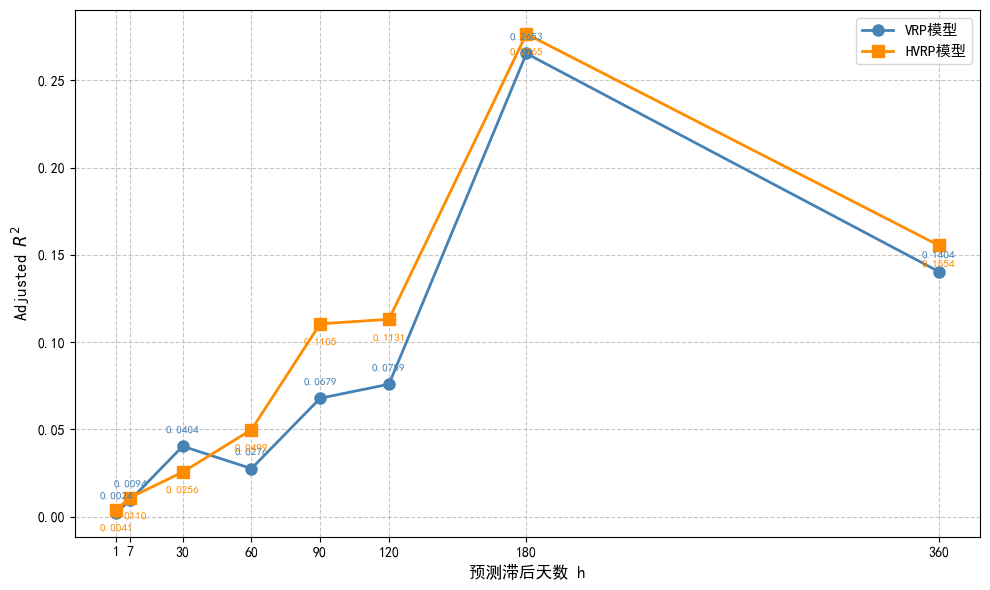
\includegraphics[width=0.9\linewidth]{r2.png}
    \caption{Comparison of Adjusted $R^2$ Values: Baseline vs. HAR-VRP Models}
    \label{fig:r2_comparison}
\end{figure}

\section{Conclusions}

Utilizing high-frequency 5-minute intraday returns and daily option trading data for the CSI 300 ETF from January 2020 to October 2025, this study systematically investigates the pricing of volatility risk in the Chinese market. By examining the term structure dynamics and asymmetric effects of the Volatility Risk Premium (VRP), and integrating the Heterogeneous Autoregressive (HAR-RV) framework for methodological refinement, we provide new evidence on return predictability. Our primary findings are summarized as follows:

First, we document a distinctive intertemporal ``sign-reversal'' in the VRP's predictive power across the term structure. In the medium-term horizon (30--90 days), the VRP exhibits a significant positive relationship with future returns, consistent with the risk-compensation hypothesis where investors demand a premium for bearing variance uncertainty. Crucially, this relationship reverses at longer horizons ($h \ge 120$), where the VRP becomes a significant negative predictor ($p < 0.001$). This robust ``positive-to-negative'' transition suggests that while the medium-term VRP predominantly reflects risk pricing, the long-term VRP captures market sentiment overreaction and subsequent mean reversion.

Second, there is a pronounced asymmetry in the predictive power of decomposed VRP components. While the upside risk premium ($VRP^+$) maintains stable and significant negative predictability for long-term horizons up to 360 days, the predictive efficacy of the downside premium ($VRP^-$) dissipates rapidly beyond the 180-day mark. This asymmetry implies that in China's evolving derivatives market, information regarding downward volatility expectations is integrated or decays more swiftly than that of upward volatility shocks, providing a critical reference for horizon-dependent market-timing strategies.

Third, the methodological refinement via the HAR-RV framework significantly enhances predictive accuracy. By incorporating daily, weekly, and monthly volatility components, the HAR-RV model filters out transitory high-frequency noise and captures the underlying structural persistence of market risk. Empirical results indicate that the refined HAR-VRP consistently outperforms traditional measures, with the Adjusted $R^2$ peaking at the 180-day horizon. This underscores the necessity of accounting for the heterogeneous nature of realized volatility when constructing forward-looking risk proxies.

Fourth, option-implied metrics demonstrate superior informational efficiency compared to volume-based indicators. Across all long-term horizons, variables derived from implied volatility—including the VIX index, mean implied volatility, and IV skewness—exhibit robust and stable predictive power. In contrast, volume-based metrics such as the call-put volume spread ($VOLD$) show only sporadic medium-term significance. This comparison confirms that the forward-looking expectations embedded in option prices are the primary drivers of long-term return predictability in the Chinese A-share market.

In summary, this study provides a comprehensive framework for pricing volatility risk in China. The identified term structure and asymmetric effects offer valuable insights for institutional investors in portfolio optimization and for regulators in monitoring market stability within an increasingly complex financial landscape.

%\bibliographystyle{apa}%%% ====================================================================}
\bibliography{ref}
\end{document}

